\documentclass[french]{article}
\usepackage[T1]{fontenc}
\usepackage[utf8]{inputenc}
\usepackage{lmodern}
\usepackage[a4paper]{geometry}
\usepackage{babel}
\usepackage[cache=false]{minted}
\usepackage{graphicx}

\title{Rapport Développement Logiciel}
\author{Badr YOUBI IDRISSI}

\begin{document}
	
\section{Introduction et fonctionnement général}

Dans ce projet nous codons un programme pour visualiser les isolignes 
d'un signal émit de plusieurs tétraèdres. Voici un schéma du fonctionnement
général :

\begin{center}
	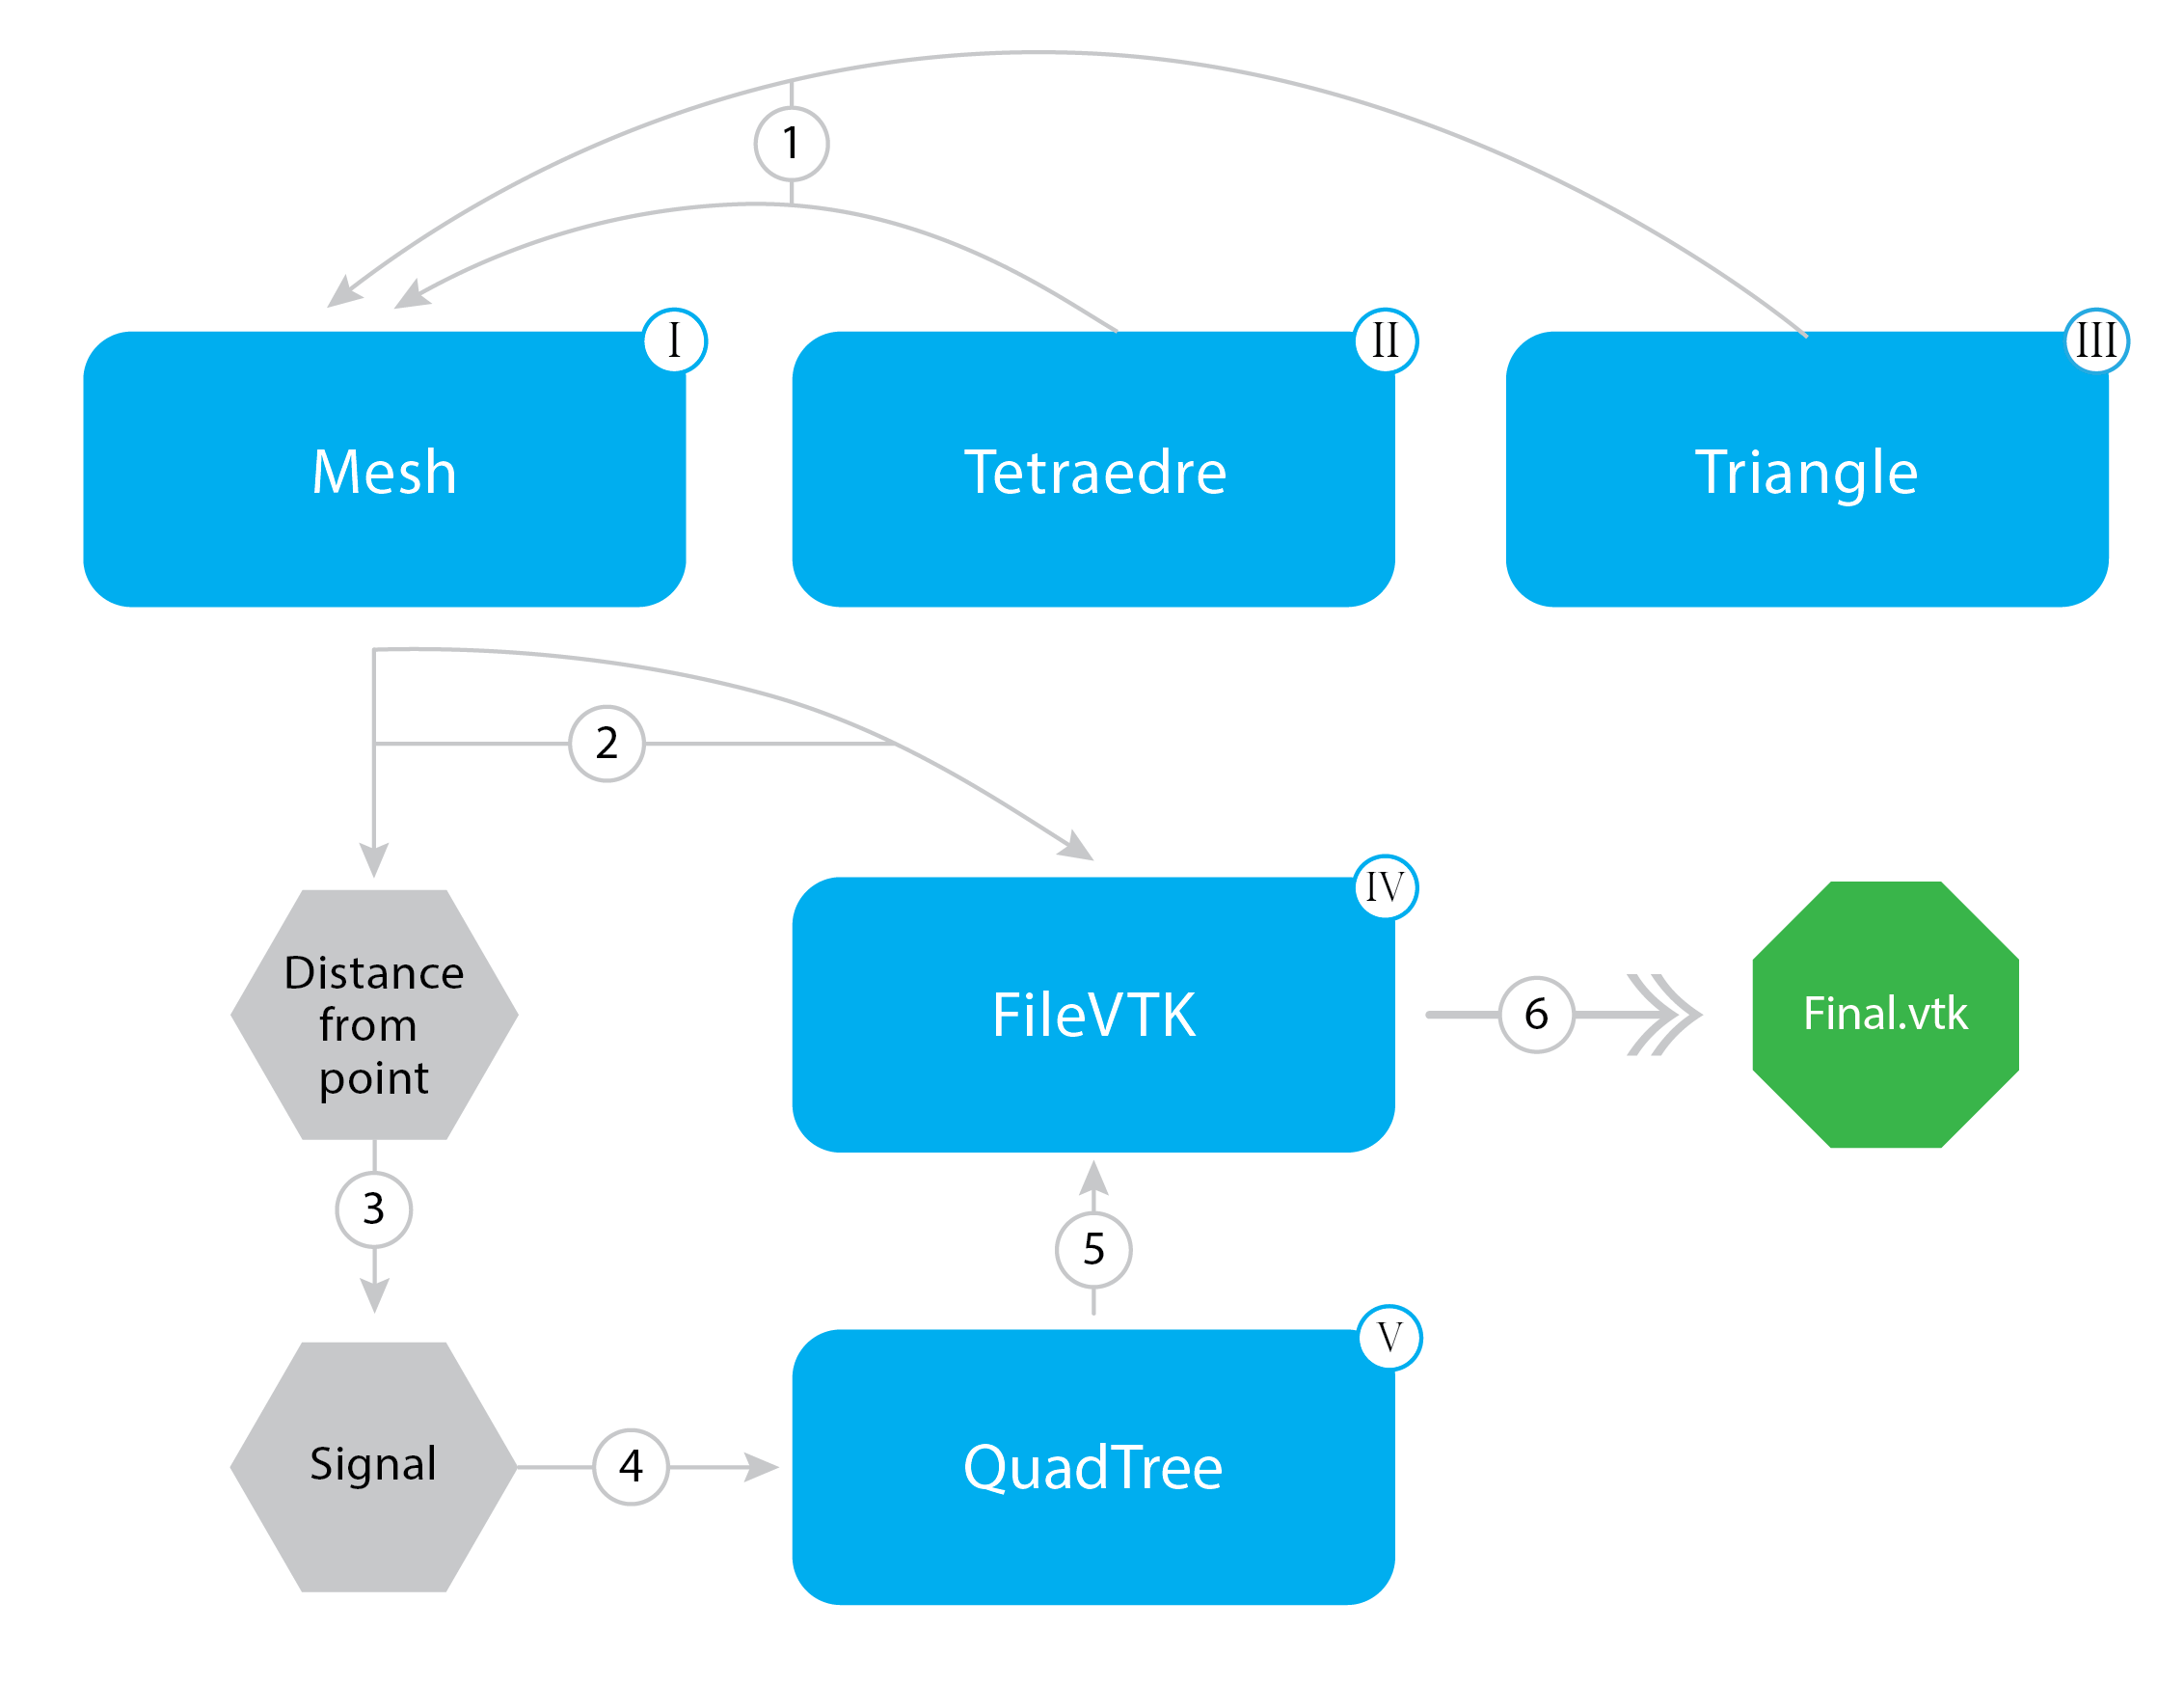
\includegraphics[width=0.7\textwidth]{Figures/SchemaNum.png}
\end{center}

On commence par créer l'objet 'Mesh' (\textit{I}) qui correspond à l'ensemble des pods émétant le signal.
L'objet mesh a besoin des points correspondant à chaque pod qui est un 'Tétraèdre' (\textit{II}) qui lui
même est un ensemble de 'Triangles' (\textit{III}) (\'Etape 1). Cet objet Mesh a la méthode distance from point qui 
renvoie la liste des distances entre un point et les pods (\'Etape 2). Ces distances servent ensuite à calculer le signal
en tout point de l'espace (\'Etape 3). on crée ensuite un plan à la hauteur 0.01 dont on va rafiner le maillage
avec l'objet 'QuadTree' (\textit{V}) (\'Etape 4). Ensuite l'ensemble des points et les valeurs du signal en ces points est
passé à l'objet 'FileVTK' (\textit{IV}) (\'Etape 5) qui va écrire le fichier "Final.vtk" (\'Etape 6).

\section{Description du code}
	
\subsection{Main}
\begin{minted}{python}
def signal(p, dico):
	outside, d_min = dico['defZone'].Distance_Between_a_Point_and_the_Modules(p)
	if outside:
		return sum(1/d_min)
	else:
		return 2*max(isoligne)
\end{minted}

\end{document}
